\subsection{Line Luminosities and Equivalent Widths}\label{sec:PhotProp.lines}
\begin{figure*}
	\centering
	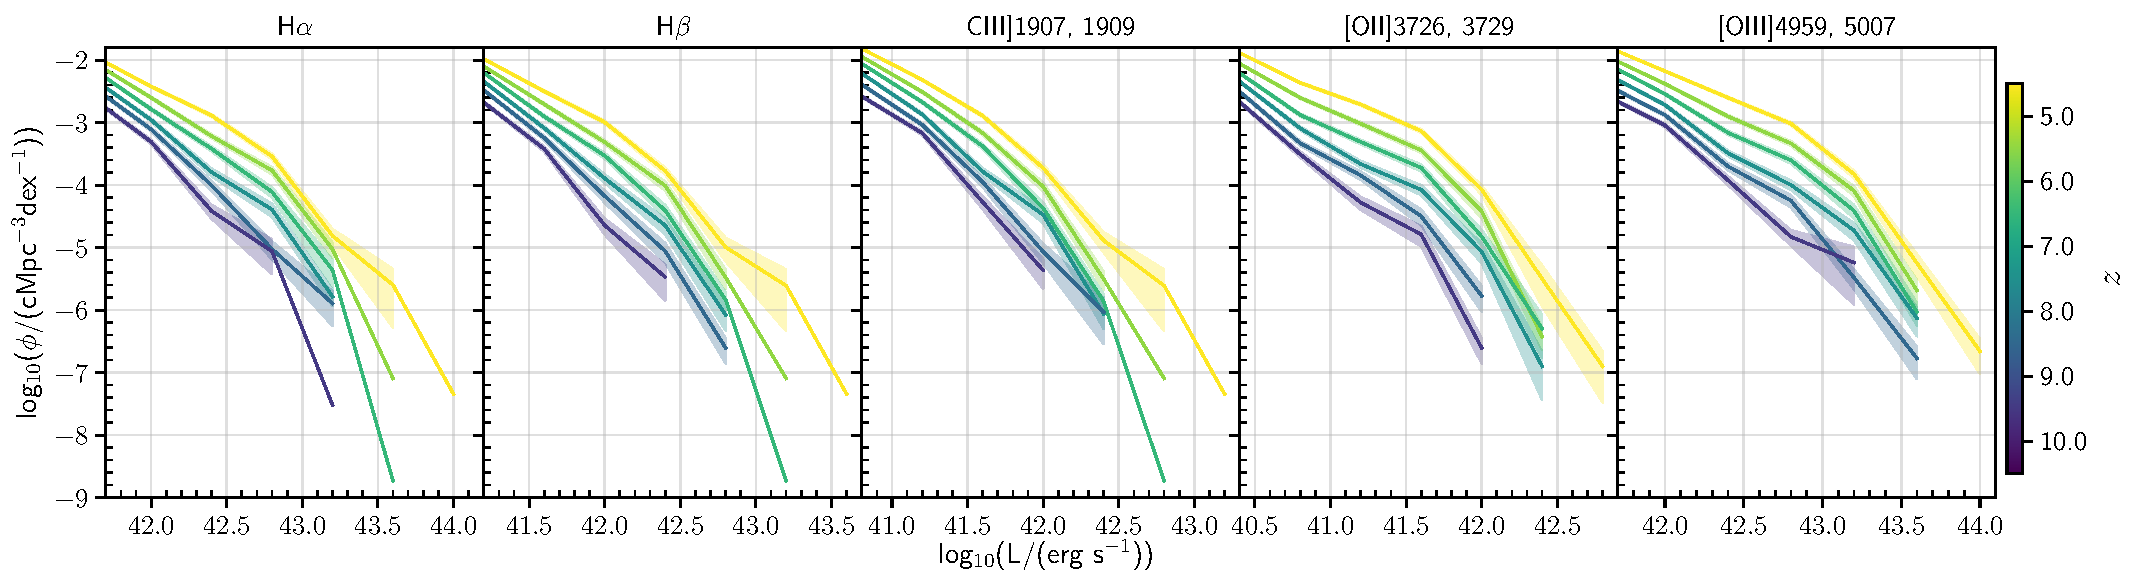
\includegraphics[width=\textwidth]{./figures/LFlines_stamps}
	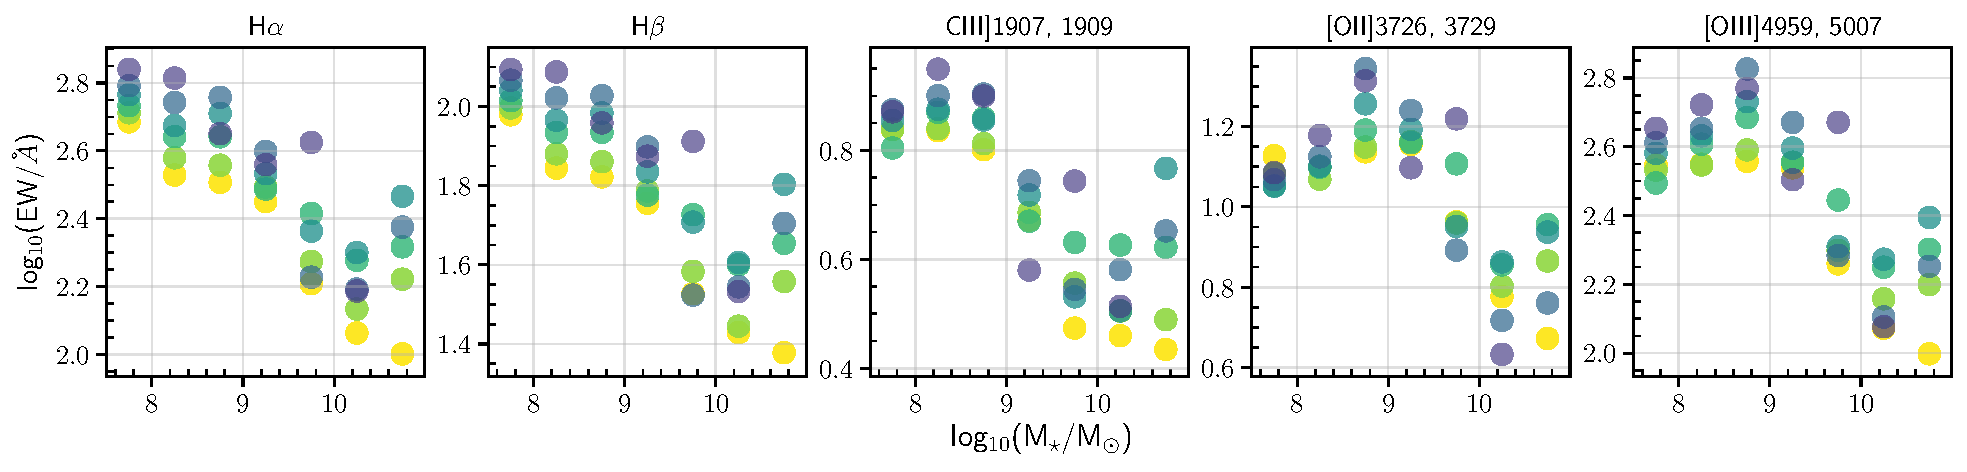
\includegraphics[width=\textwidth]{./figures/EWlinesMstar_stamps}
	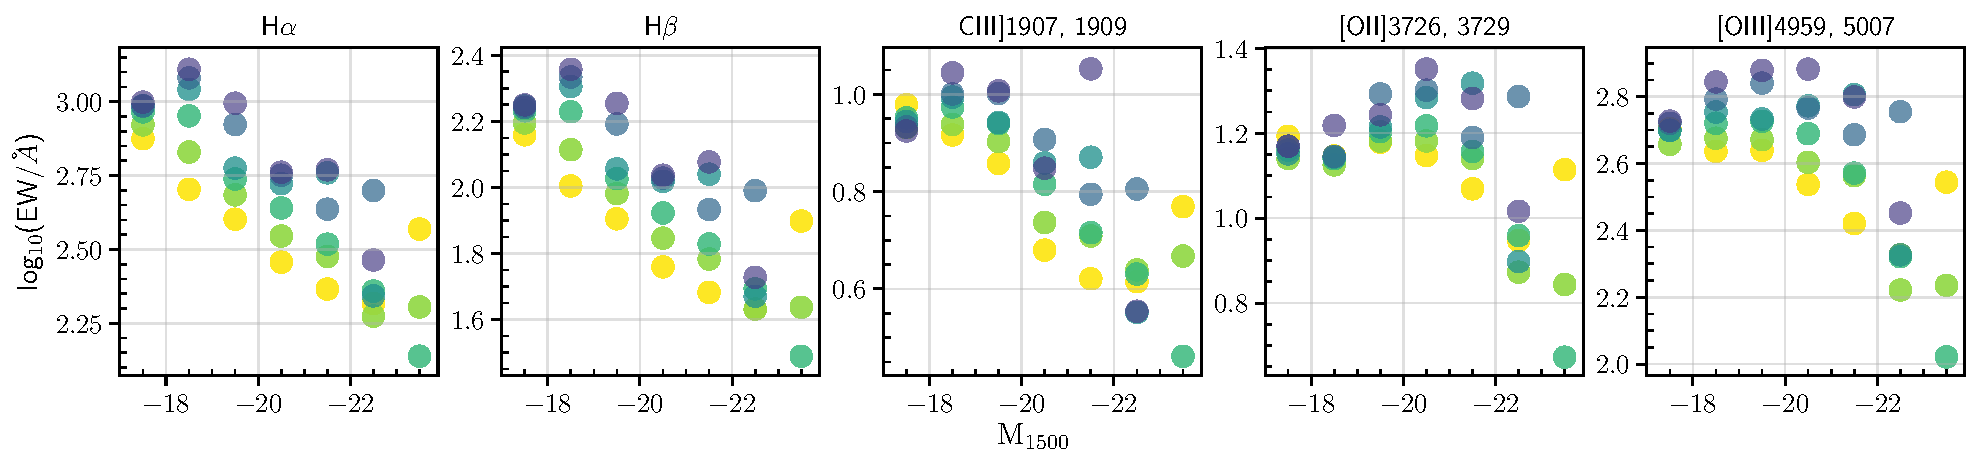
\includegraphics[width=\textwidth]{./figures/EWlineslum_stamps}
	\caption{Predictions for the properties of 6 prominent UV and optical lines in \flares\, for $z\in[5,10]$. The colour bars for the different redshifts are shown in the rightmost panel. In the top panel we show the dust-attenuated luminosity functions for each line, with the shaded region representing the 1$\sigma$ poisson uncertainties. Middle panel shows the evolution of the weighted median equivalent widths of these lines in stellar mass bins. Bottom panel shows the weighted median equivalent widths as a function of FUV luminosity. \label{fig: LF_line_evo}} 
\end{figure*} 
\begin{figure*}
	\centering
	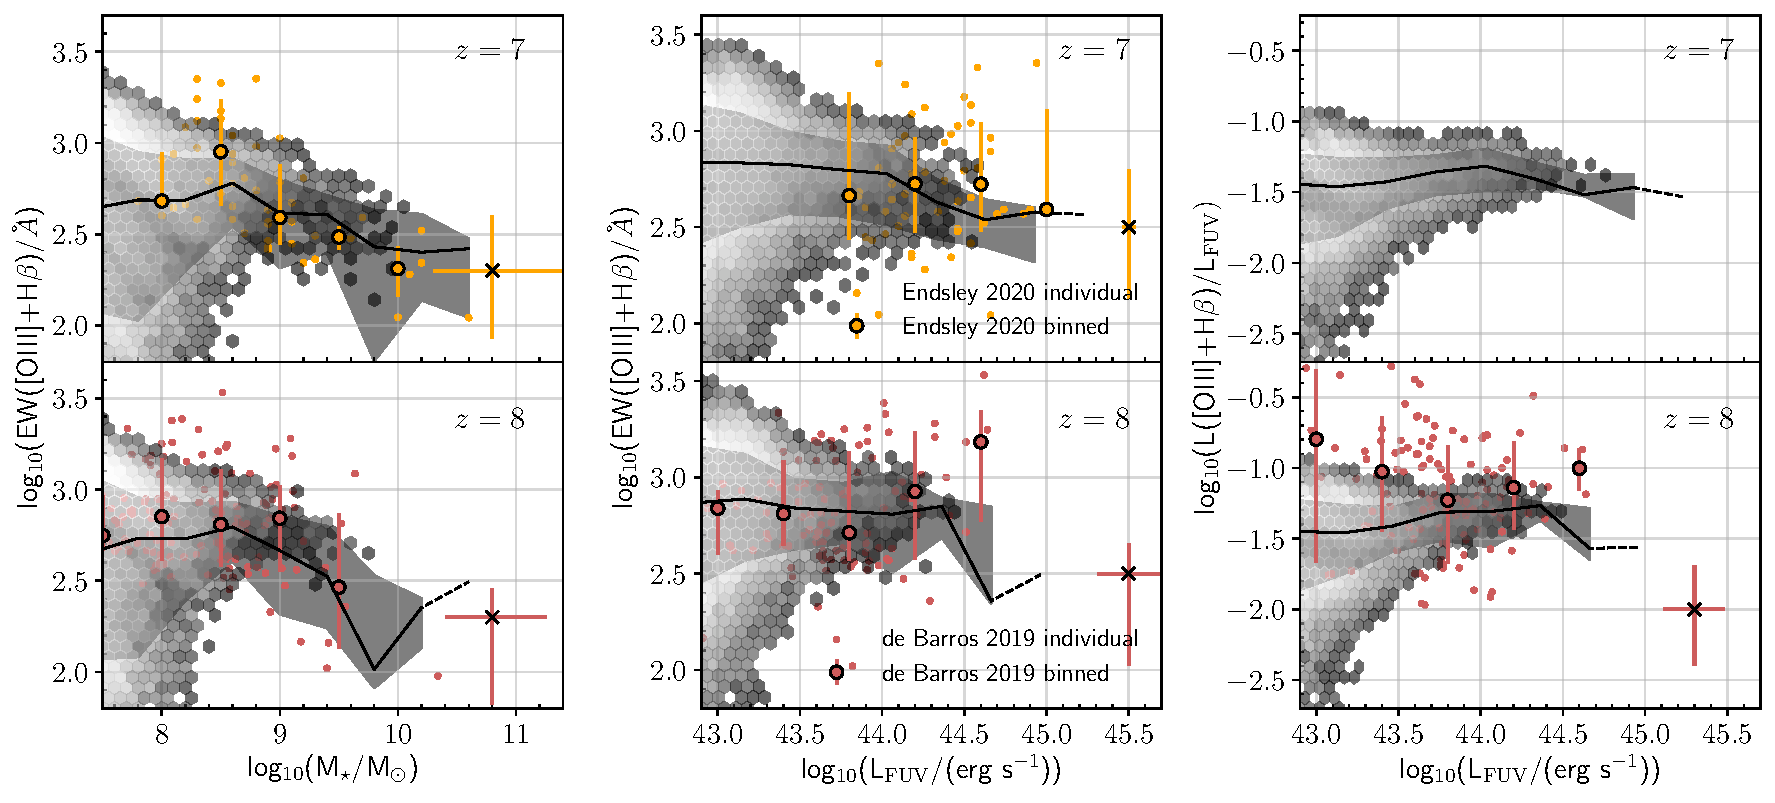
\includegraphics[width=\textwidth]{./figures/line_lum_z7_8}
	\caption{Left: Predicted distribution of combined H${\beta}$ and [OIII]$\lambda$4959,5007 equivalent widths and stellar masses for \flares\, galaxies at $z\sim7,8$. Middle: Predicted distribution of combined H${\beta}$ and [OIII]$\lambda$4959,5007 equivalent widths to the far-UV luminosity of \flares\, galaxies at $z\sim7,8$. Right: Predicted distribution of the H${\beta}$ and [OIII]$\lambda$4959,5007 line luminosities to the far-UV luminosity and far-UV luminosities of \flares\, galaxies at $z\sim7,8$. The solid dashed line is the weighted median of the sample, with the shaded region indicating the weighted 84 and 16 percentiles. The hexbin denotes the distribution of our sample, only plotted are bins with more than 5 data points. The small circles show the individual measurements from \protect\cite{deBarros19_OIIIHbeta,Endsley2020} while the large points denote the median value in bins of stellar mass and far-UV luminosities respectively. The errorbars centered on the cross shown at the bottom-right gives the median errors on the observational data.\label{fig: OIII_z7_8}} 
\end{figure*} 
\begin{figure}
	\centering
	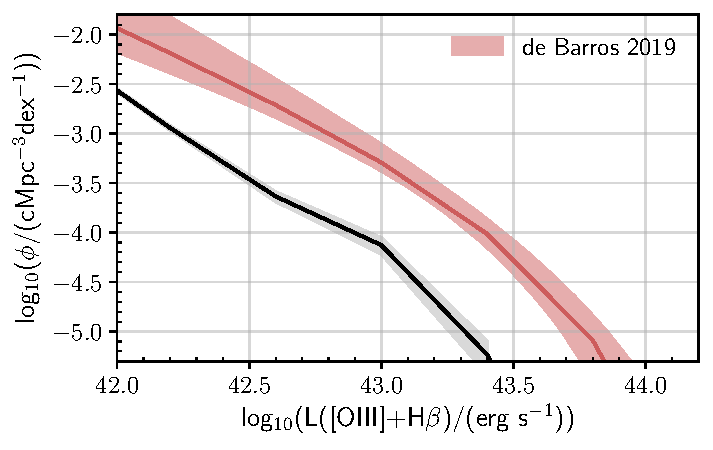
\includegraphics[width=\columnwidth]{./figures/LFOIII_z8}
	\caption{The \protect\cite{deBarros19_OIIIHbeta} and predicted combined H$\beta$ and [OIII]$\lambda$4959,5007 line luminosity function of \flares\, galaxies at $z\sim8$. \label{fig: OIII_LF_8}} 
\end{figure}
%		
%		CIII]1909 and Lyman-alpha or metallicity comparison?
	
In this section we will present some of the nebular emission line properties and compare them to some of the available observational constraints. 
 
We present predictions for 6 prominent nebular lines or doublets in the UV in Figure~\ref{fig: LF_line_evo}. The top panel shows the evolution of the line luminosity function with redshift, for $z\in[5,10]$. The overall shape of the function is similar to the UV luminosity function of galaxies and can be approximated by a Schechter function at these redshifts. The LF of the lines evolves with redshift, with almost 3 dex in value near the knee of the function. Also presented is the predictions for the evolution of the weighted median equivalent widths of these lines as a function of stellar mass (middle panel) and far-UV luminosity (bottom panel) with redshift in Figure~\ref{fig: LF_line_evo}. For galaxies with similar stellar mass the equivalent width mostly increases with increasing redshift, indicating that they have harder ionising photons from their younger stellar population with more massive stars. There is also the effect of metallicity on the line width, causing them to drop quickly at higher stellar masses in case of the hydrogen recombination lines, while the other lines peak around 10$^9$M$_{\odot}$ and then fall rapidly. In case of the far-UV the relationship between with metallicity is not correlated in the same way as stellar mass and hence intepretation is harder. But in most cases this also shows increasing equivalent widths at higher redshifts for fixed far-UV luminosity. 

Both \cite{deBarros19_OIIIHbeta,Endsley2020} have combined broadband photometry from \textit{Hubble} and \textit{Spitzer} observations to constrain the prominent H$\beta$ and [OIII]$\lambda$4959,5007 lines at $z\sim 7,8$. In Figure~\ref{fig: OIII_z7_8} we plot the combined values of [OIII]$\lambda$4959,5007 and H$\beta$ line luminosities as well as the equivalent widths (EWs) of \flares\, galaxies at $z=7,8$ against these observational data sets. As can be seen from the figure, in the case of the equivalent width measurements plotted against the stellar mass (left panel) or FUV luminosity (middle panel) of the \flares\, galaxies, the weighted median closely follows the observations. However, it should be noted that our modelling does fail to reproduce some of the larger values of the EW measurements. In case of the line luminosity normalised by the far-UV luminosity (right panel), the \flares\, data lies $\sim 0.3$ dex below the observational data from \cite{deBarros19_OIIIHbeta}. The effect of under-predicting these observations is also seen in the [OIII]$\lambda$4959,5007 luminosity function as predicted by \cite{deBarros19_OIIIHbeta}, where the \flares\, result is offset by $\approx0.6$ to lower number densities or by $\approx0.4$ to lower luminosities. The implications of this is that the observations measure higher dust attenuation compared to \flares\, and particularly in case of the line luminosity function the discrepancy might be due to the relation used by \cite{deBarros19_OIIIHbeta} to convert the observed far-UV LF to a line luminosity LF. Other possibilities of discrepancy lies in the intrinsic physical properties of the galaxies like the stellar age and metallicity, as well as assumption in the nebular emission modelling like the nebular hydrogen density or ionisation parameter \citep[see][]{Wilkins2020}. Future direct emission line measurements from \jwst\, and other facilities will help to constrain this observational space and thus better understand this discrepancy. %\jwst\ also has access to the Paschen line series, which suffers less attenuation than the H$\beta$ and thus can be intrumental for attenuation corrections.

%~~~~~~Calibration relations for SFR vs line luminosity?~~~~~~
%With the \flares\, galaxies matching most of these high redshift line luminosity observations, we present scaling relations to measure the star formation rate of galaxies from some of the line emissions availabe at high redshift. H$_{\alpha}$, H$_{\beta}$, some [OIII] or [OII]3727,3729 lines? Comparison to Kennicut relations?